
\section{Scopo e strumentazione}
Scopo dell'esercitazione è verificare i vari regimi di funzionamento di un transistor BJT. Si misurano i parametri rilevanti di tale componente come il guadagno in corrente . Si usa il transistor come amplificatore di corrente e come commutatore per realizzare un circuito not.

\section{Materiali}
Si è analizzato il funzionamento di un transistor 2N17711. Da datasheet si legge:

\begin{itemize}
\item massima tensione collettore-base: $75 V$
\item massima tensione collettore-emettitore: $50 V$
\item massima tensione base-emettitore: $7 V$
\item massima corrente di collettore: $500 mA$
\item massima potenza dissipata: circa $1 W$
\end{itemize}
Per come è pensato l'esperimento non è previsto andare oltre questi limiti. 


\section{Misure in DC sul transistor}
\subsection{b}
Si è monatato il circuito in figura (\ref{f:circuito DC}).Per le caratteristiche del circuito ($V_1\simeq \SI{10}{\volt}$, $R_1\simeq \SI{1}{\kilo\ohm}$) si ottiene la retta di carico in \fig{retta di carico}
\begin{figure}
	\centering
	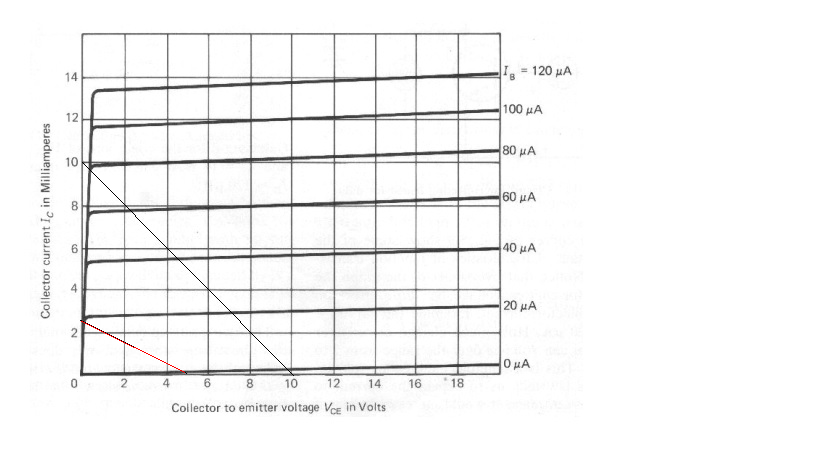
\includegraphics[scale=0.4]{retta_di_carico.png}
	\caption{Retta di carico e curve tensione corrente.\label{f:retta di carico}}
\end{figure}

\begin{figure}
	\centering
	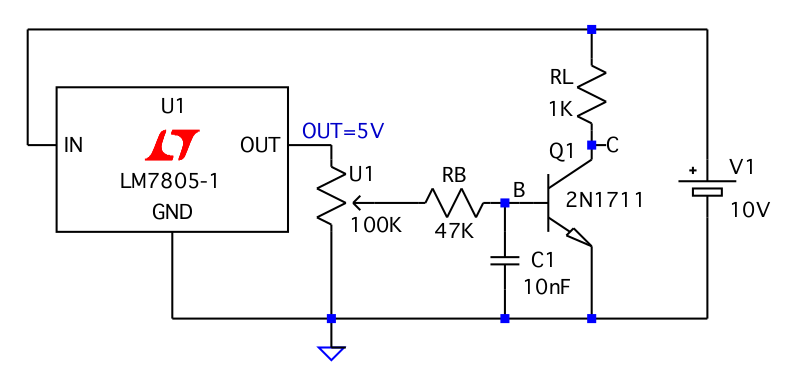
\includegraphics[scale=0.4]{circuito_DC.png}
	\caption{Circuito usato nella prima parte dell'esperienza .\label{f:circuito DC}}
\end{figure}



\subsection{c}
Si è misurata la corrente di collettore in funzione della corrente e della tensione di base (corrente di base misurata attraverso la caduta di potenziale su $R_B$, corrente di collettore attraverso la caduta su $R_L$); i dati sono riassunti in \tab{Ic_vs_Ib_vs_Vb}. In \fig{fit1} si possono vedere i dati sperimentali della corrente di collettore in funzione della corrente di base. Le rette verde e rossa sono i rispettivi fit in regione attiva e regione di saturazione. Gli errori riportati dal grafico sono solo quelli di lettura. Per procedere con il fit solo questi sono stati considerati casualmente indipendenti, dunque utilizzati per la minimizzazione del $\chi^2$.

\begin{figure}
	\centering
	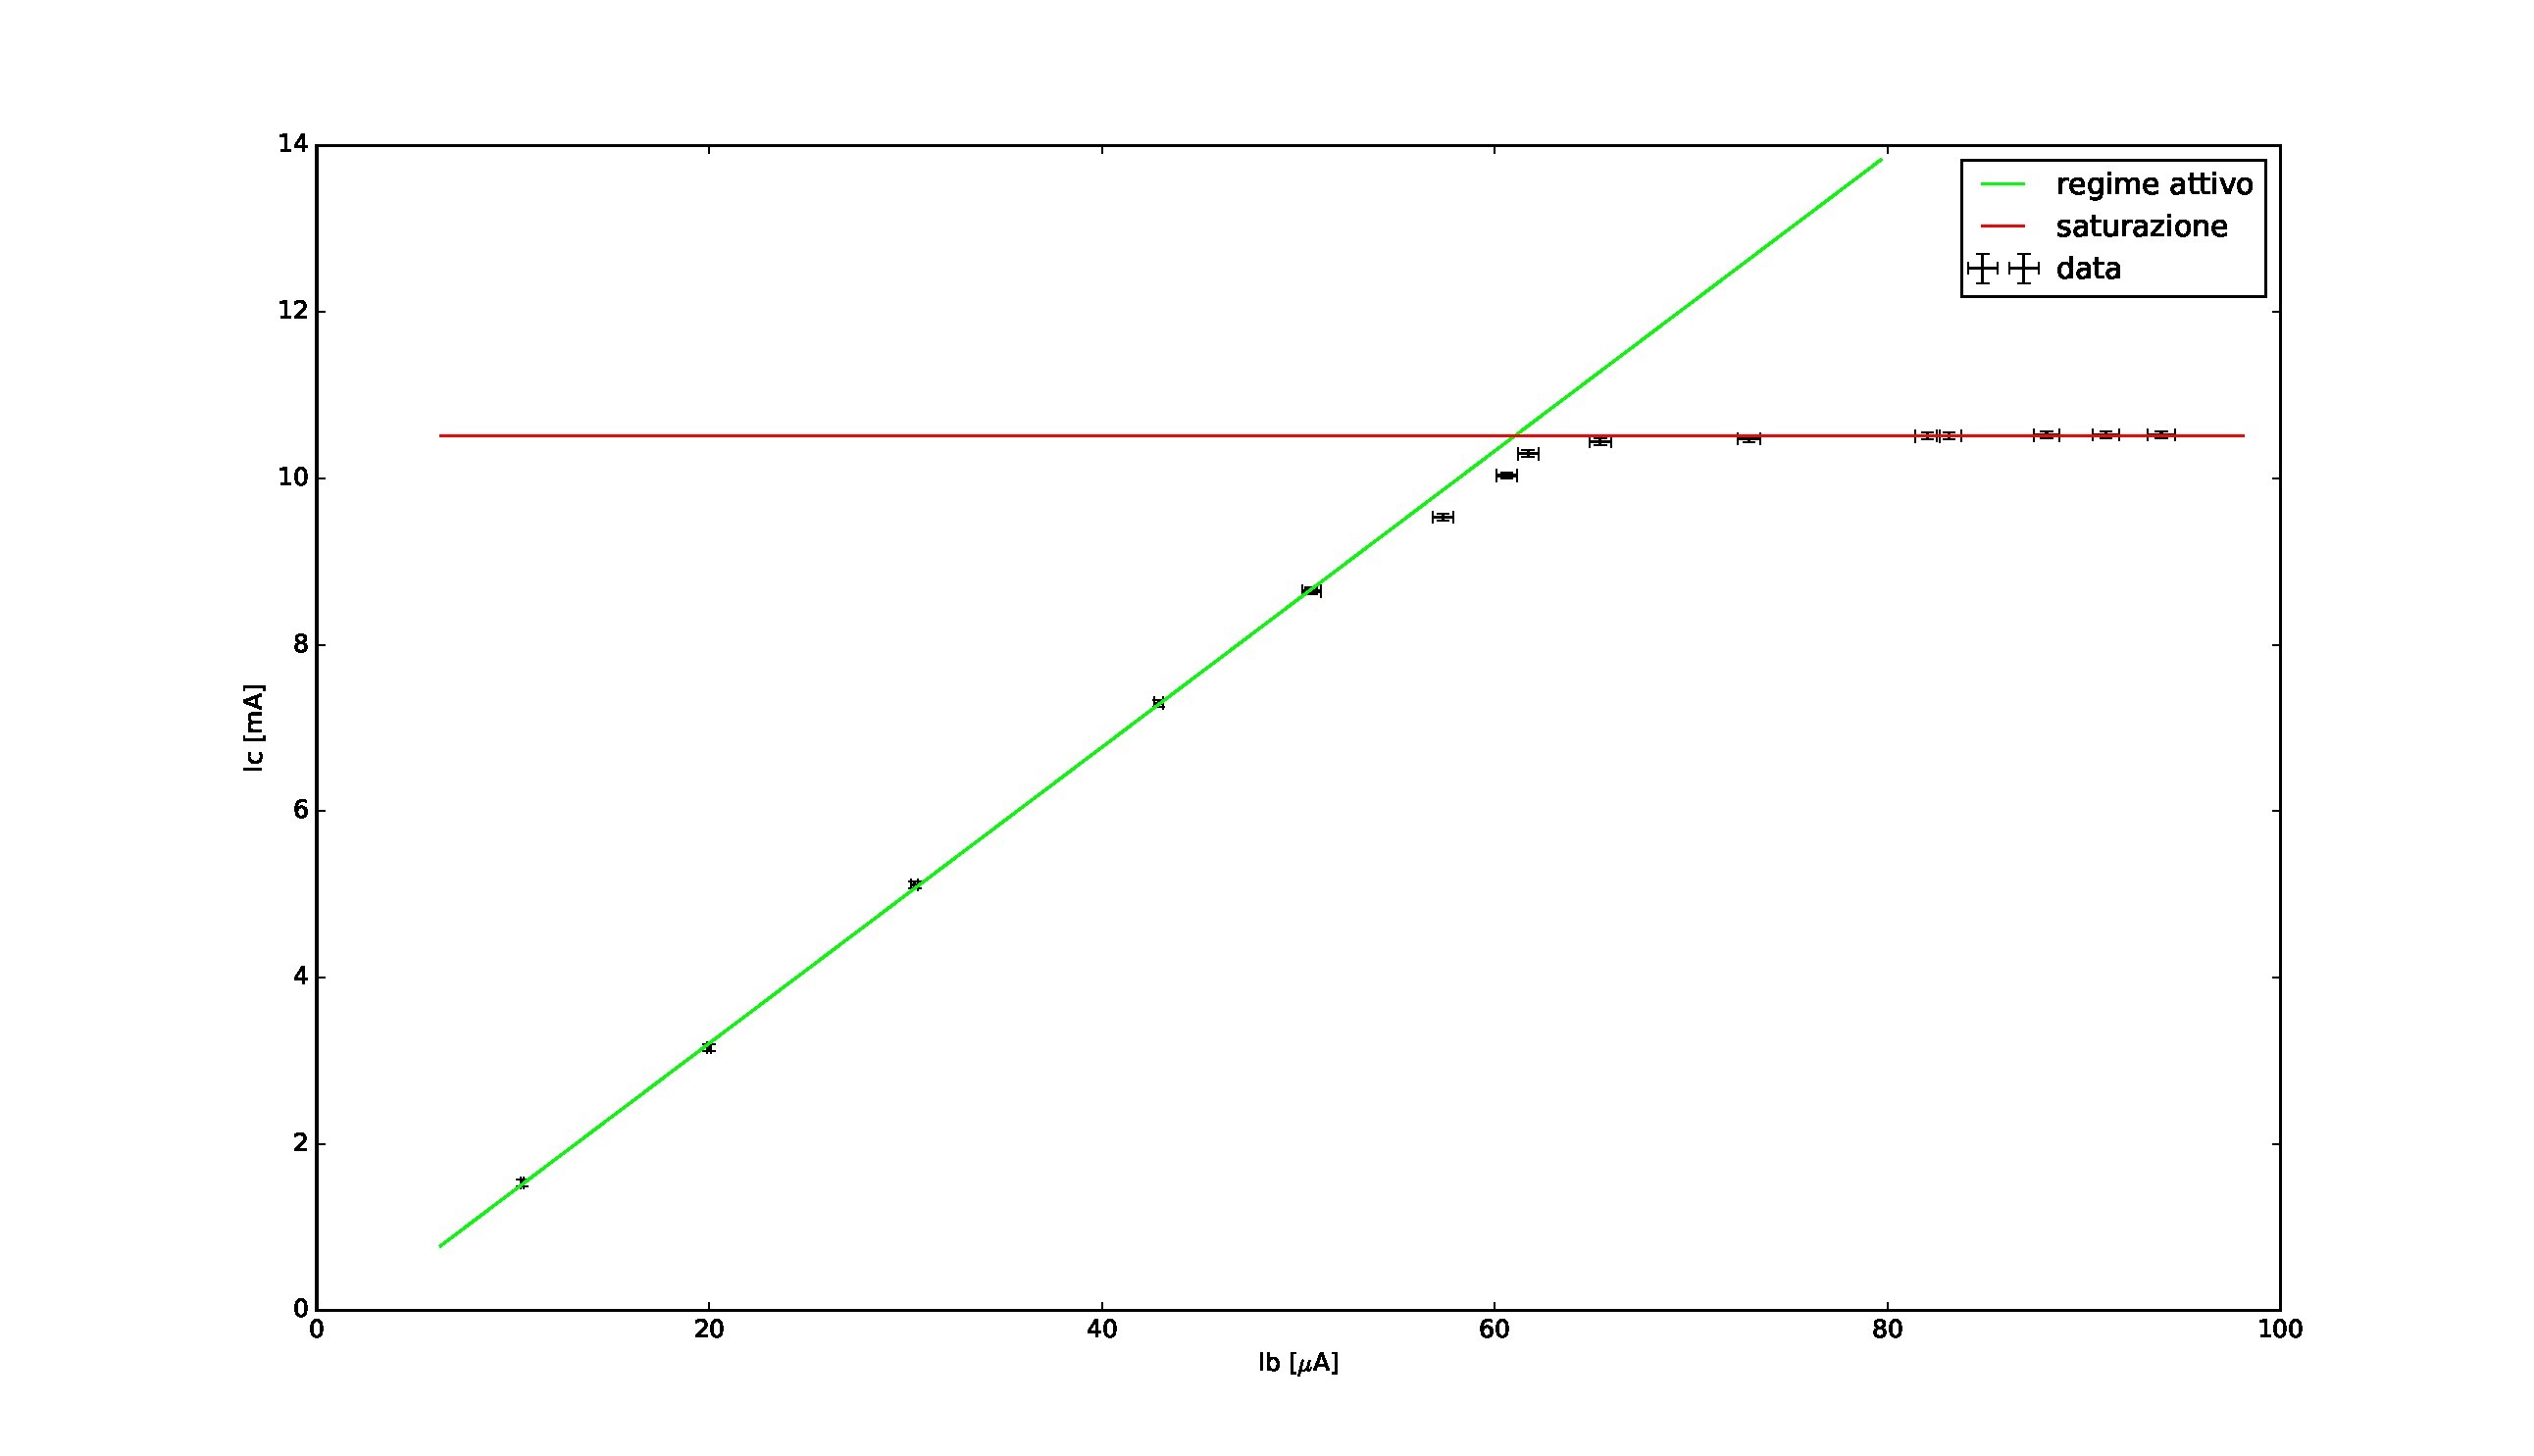
\includegraphics[scale=0.3]{plot5c_lines.pdf}
	\caption{Fit di corrente di saturazione e di Ic vs Ib in zona attiva.\label{f:fit1}}
\end{figure}

\begin{table}
	\centering
	\begin{tabular}{S[table-figures-decimal = 2, table-figures-uncertainty = 3] S[table-figures-decimal = 0, table-figures-uncertainty = 1] S[table-figures-decimal = 2, table-figures-uncertainty = 3]} 
		$I_b$ [\si{\mA}]	&	$V_{be}$ [\si{\mV}]	&	$I_c$ [\si{\uA}]	\\
		\hline 
		10.48 (7)	&	604 (4)	&	1.53 (4)	\\ 
		19.98 (12)	&	620 (4)	&	3.16 (4)	\\ 
		30.45 (17)	&	636 (4)	&	5.12 (4)	\\ 
		42.88 (23)	&	644 (4)	&	7.30 (4)	\\ 
		50.6 (4)	&	652 (4)	&	8.64 (4)	\\ 
		57.4 (5)	&	664 (4)	&	9.53 (4)	\\ 
		60.6 (5)	&	668 (4)	&	10.03 (4)	\\ 
		61.7 (5)	&	660 (4)	&	10.30 (4)	\\ 
		65.4 (5)	&	668 (4)	&	10.44 (4)	\\ 
		72.9 (5)	&	672 (4)	&	10.48 (4)	\\ 
		82.0 (6)	&	672 (4)	&	10.51 (4)	\\ 
		83.1 (6)	&	668 (4)	&	10.51 (4)	\\ 
		88.1 (6)	&	672 (4)	&	10.52 (4)	\\ 
		91.1 (6)	&	672 (4)	&	10.52 (4)	\\ 
		93.9 (6)	&	672 (4)	&	10.52 (4)	\\ 
		\end{tabular} 
	\caption{Dati raccolti variando la posizione del potenziometro. \label{t:Ic_vs_Ib_vs_Vb}} 
\end{table}


Il fit in regione attiva è una retta affine ($I_c = h_{fe} I_b + K_0$, 2 parametri). Si sono tagliati arbitrariamente i dati considerati in regione attiva a \SI{55}{\micro\ampere}. Le caratteristiche fittate sono le seguenti: \\
$h_{fe}=178  \pm 3 \\
K_0=-0.35 \pm 0.05 mA$

La correlazione lineare fra i due parametri è di $0.8$, il $\chi^2=3.25 (3\dof)$.

I risultati meritano un commento. In prima battuta si può pensare che $K_0$ non sia compatibile con zero, ma alle misure fatte vanno ancora aggiunti gli errori sistematici. In particolare:\\
$R_B=46.2 \pm 0.5 kOhm$\\
$R_L=981\pm 9 Ohm$\\
errore calibrazione oscilloscopio: $3\%$ \\
Propaghiamo dunque gli errori di calibrazione su questi parametri. Essendo $h_fe=I_c/I_b$ basterà sommare in quadratura gli errori relativi su $I_c$ e $I_b$ (se ne prenderà un valore medio nel campione). Questo da un $6\%$ di errore di calibrazione sul $h_{fe}$, che sommato (sempre in quadratura) con il risultato del fit:\\
 $h_{fe}=178\pm 10$\\
Per $K_0$ bisogna procedere similmente. Le correnti $I_c$ hanno un errore di calibrazione del $5\%$, dunque in media ($6 m A$) nel campione un errore di $0.3 m A$.
$K_0=-0.35 \pm 0.3 mA$. 
Si può procedere similmente per la zona di saturazione. Questa volta si è preferito fittare la retta costante(1 parametro), scegliendo come corrente di base di taglio $70 \mu A$. I risultati del fit sono:\\
$I_{c(sat)}= \SI{10.51 (2) }{\mA}$\\
con un $\chi^2=0.8 (5 \dof)$.
L'errore va naturalmente trattato come prima. In pratica si aggiunge un errore del \SI{5}{\percent}. Dunque:\\
$I_{c(sat)}=10.5 \pm 0.5 mA$\\
Chiaramente il $\chi^2$ così basso non permette di dare significato statistico al primo errore dato.

Dal valore ottenuto per $I_{c(sat)}$, unitamente ai valori misurati per $V_{cc}$ e $R_L$ (rispettivamente \SI{10.46(4)}{\V} e \SI{981(9)}{\ohm}), si ricava il valore di $V_{ce}$ in sona di saturazione: \\
$V_{ce(sat)} = V_{cc} - R_L I_{c(sat)} = \SI{0.15(10)}{\V}$

La corrente $I_c$ massima erogabile dal transistor è data dall'intersezione tra la retta di carico e le curve caratteristiche del transistor in zona di saturazione; approssimando queste ultime a rette verticali (approssimazione non valida se si intende lavorare su rette di carico molto distanti, e in particolare molto più basse, di quella determinata dal circuito usato) $V = V_{ce(sat)}$ si ha, in funzione delle altre caratteristiche del circuito, $I_{max} = \frac{V_{cc} - V_{ce(sat)}}{R_L}$.

\subsection{e}
Al variare della tensione di alimentazione $V_{cc}$ la retta di carico viene traslata verticalmente: ci aspettiamo dunque che mantenendo $I_b$ costante il punto di lavoro si sposti al variare di $V_{cc}$ lungo la curva caratteristica corrispondente (che in zona attiva ci attendiamo sia approssimabile a una retta dal basso coefficiente angolare).

Portandoci a $I_b = \SI{33.8 (4)}{\uA}$ (in pieno regime attivo secondo quanto visto precedentemente), si sono presi al variare di $V_{cc}$ i dati in \tab{dati_5e}, riassunti dal grafico in \fig{5e_Vearly}; è stata poi fittata una retta (2 parametri) la cui intersezione con l'asse delle ascisse dà il valore di $V_{Early}$ (l'errore è stato trattato come nei fit precedenti): si sono ottenuti valori di \SI{82(19)}{\micro\A\per\volt} per il coefficiente angolare e \SI{5.41(5)}{\milli\ampere} per l'intercetta (coefficiente di correlazione $-0.75, \ \chi^2 = 14 \ (8 \dof)$), che danno per $V_{Early}$ un valore di \SI{-66 \pm 16}{\V}. Il $\chi^2$ relativamente alto e l'andamendo particolare dei dati nel grafico sono probabilmente dovuti a effetti di dipendenza della corrente di base (e dunque quella di collettore) dalla temperatura: durante la presa dati abbiamo infatti notato che mantenendo $V_{cc}$ (e dunque di $V_{ce}$) a valori abbastanza alti (ma pur sempre entro i \SI{15}{\V}) la caduta di tensione su $R_B$, e con essa la corrente $I_b$ variava in modo non trascurabile (0.5-1\si{\percent}), il che abbiamo ritenuto essere attribuibile la variazione delle caratteristiche del circuito in seguito al leggero riscaldamento dei componenti attivi. Abbiamo cercato di minimizzare questo effetto (che ci avrebbe essenzialmente portato a prendere dati su curve caratteristiche relative a $I_b$ diverse) alternando misure a $V_{cc}$ più bassi e più alti, riuscendo a mantenere le variazioni di $V_{R_B}$ sempre entro 1 digit della misura effettuata con il multimetro ($\lesssim \SI{0.1}{\percent}$), ma questo potrebbe non essere stato sufficiente.

\begin{figure}
	\centering
	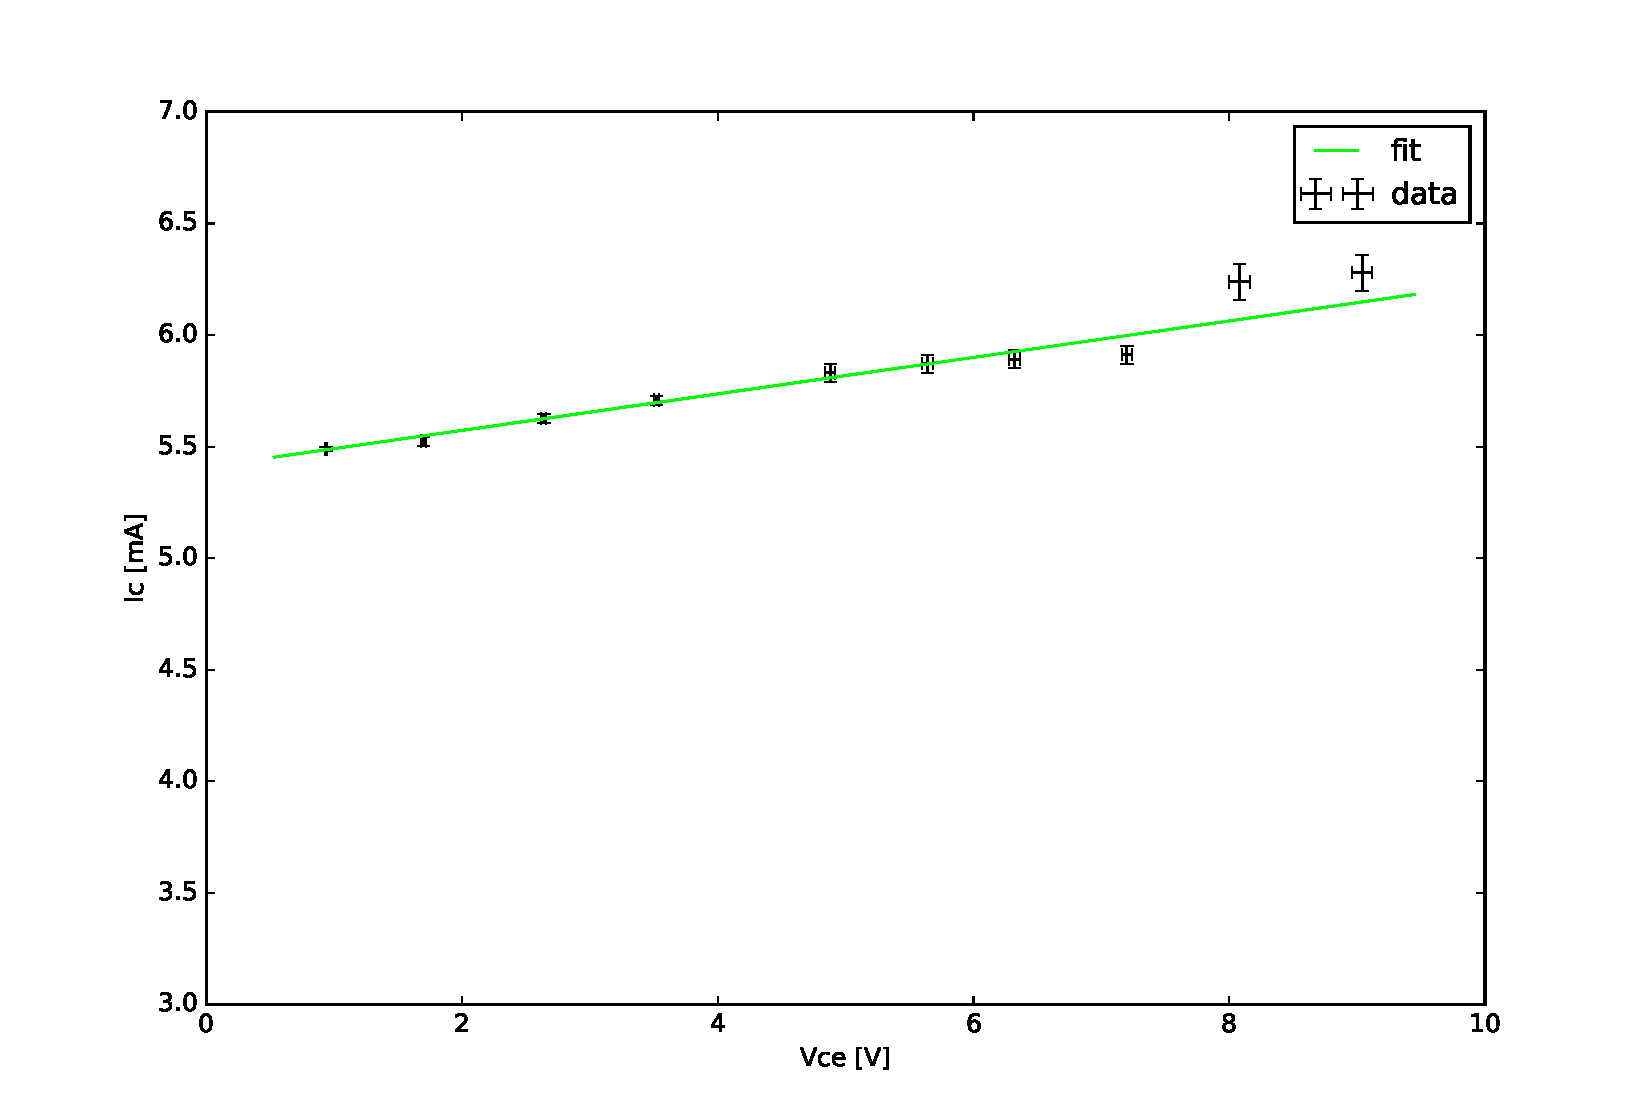
\includegraphics[scale=0.6]{5e_Vearly.pdf}
	\caption{Fit della retta che approssima la curva caratteristica in zona attiva.\label{f:5e_Vearly}}
\end{figure}

\begin{table}
	\centering
	\begin{tabular}{*{2}{S[table-figures-decimal = 3, table-figures-uncertainty = 3]}} 
		{$V_{ce}$ [\si{\V}]}	&	{$I_c$ [\si{\mA}]} \\
		\hline 
		0.936 (8)	&	5.488 (8)	\\ 
		1.700 (20)	&	5.525 (20)	\\ 
		2.640 (20)	&	5.627 (20)	\\ 
		3.520 (20)	&	5.708 (20)	\\ 
		4.88 (4)	&	5.83 (4)	\\ 
		5.64 (4)	&	5.87 (4)	\\ 
		6.32 (4)	&	5.89 (4)	\\ 
		7.20 (4)	&	5.91 (4)	\\ 
		8.08 (8)	&	6.24 (8)	\\ 
		9.04 (8)	&	6.28 (8)	\\ 
	\end{tabular} 
	\caption{Dati raccolti variando $V_{cc}$ in zona attiva. \label{t:dati_5e}} 
\end{table}

\subsection{$I_c$ vs $V_b$}
Da questi dati si è provato a procedere con un fit in zona attiva (curva rossa), ma la scarsezza di punti non ha permesso di ottenere risultati soddisfacenti (tensione termica $v_t\simeq \SI{5}{\milli\volt}$). La tensione di soglia sembra essere comunque dell'ordine dei $\SI{0.6}{\V}$

\begin{figure}
	\centering
	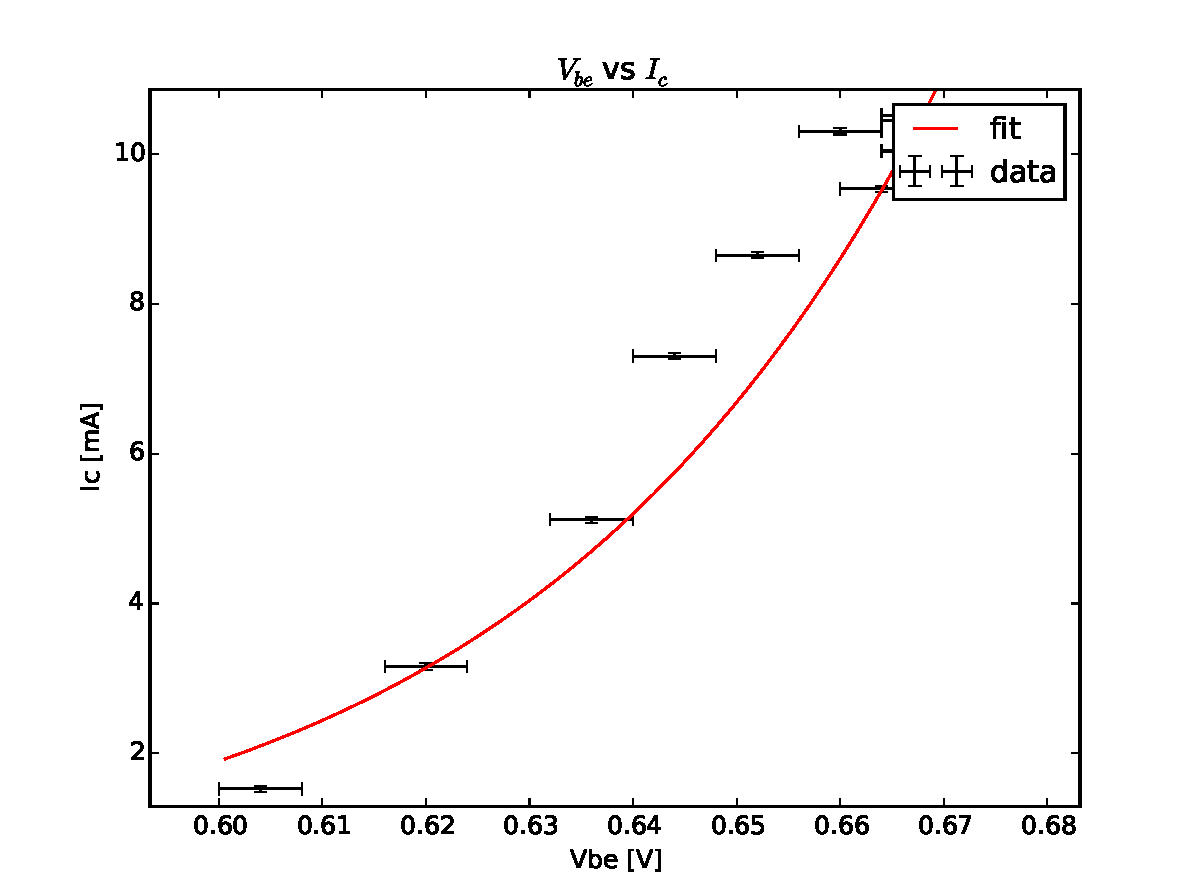
\includegraphics[scale=0.6]{malofit.pdf}
	\caption{La curva rossa non approssima bene i dati sperimentali.\label{f:schifo}}
\end{figure}
 



